\acresetall
\chapter{Background}\label{ch:background}

This chapter presents information about the relevant software and hardware. The first section gives a short introduction on virtualization and its benefits, and then describes the Xen hypervisor. The next section overviews the LibVMI \ac{API} and DRAKVUF, the library and main application we will leverage, as well as the system call functionality and convention. Finally, we review some of the existing solutions that leverage introspection.

\section{Virtualization}\label{sec:virtualization}
Running many and different services on a single \ac{OS} is an implementation method that vendors are abandoning, as mentioned in Rosenblum and Garfinkel~\cite{rosenblum2005virtual}. In the past years advances in computing have enabled users to run a plethora of different software, which became a challenge to manage efficiently and securely because each service required a specific \ac{OS} configuration. Over time hardware became inexpensive and service providers preferred to run one service per physical system to achieve higher security, since now each \ac{OS} could be configured properly for the one service it was running. On the downside, running one service per physical machine resulted in the underutilization of hardware and capabilities, as well as increased maintenance costs. Hosting different \ac{VM}s on a single and powerful system (Fig.~\ref{fig:tovirt}) solves many of the problems, as observed by Rosenblum and Garfinkel~\cite{rosenblum2005virtual}. \ac{VM}s cause resources to be used efficiently, with each service using only a part of the underlying hardware. \acp{VM} also allow easier security implementation, because it is much simpler to secure one \ac{VM} running one service, than having to combine all of them into one. Additionally virtualization achieves redundancy between services, since each \ac{VM} is independent from the rest, and any one failure does not affect the other \ac{VM}s.

\par The advantages of virtualization do not stop there. Easy backup, restore, cloning, and migration of a system are just a few of them. Creating snapshots of entire machines and restoring to a previous state, in case of corruption or misconfiguration, has become a trivial task. Also, modern hypervisors implement a very solid and sophisticated \ac{VM} isolation; pivoting from one \ac{VM} to another has become extremely difficult.

\begin{figure}
	\centering
	%\documentclass[tikz, border=10pt]{standalone}
%%%<
%%%>
\begin{comment}
:Title: Basic Philosophy concepts
:Tags: Diagrams;Graphs;Philosophy
:Author: Vilson Vieira
:Slug: philosophy

This graph diagram presents the basic Philosophy concepts of dialectics,
opposition and innovation.
\end{comment}

\def\xout{3.5}
\def\yout{2.2}
\def\xin{1.8}
\def\yin{1.05}
\def\xapp{3}
\def\yapp{1.9}
\def\xhard{-0.7}
\def\xr{0}
\def\yr{0.2}
\def\xb{4}
\def\yb{0.2}
\def\xg{2}
\def\yg{-2.5}
\def\xrr{10}
\def\yrr{1}
\def\xbb{10}
\def\ybb{-1.8}
\def\ygg{-4.6}
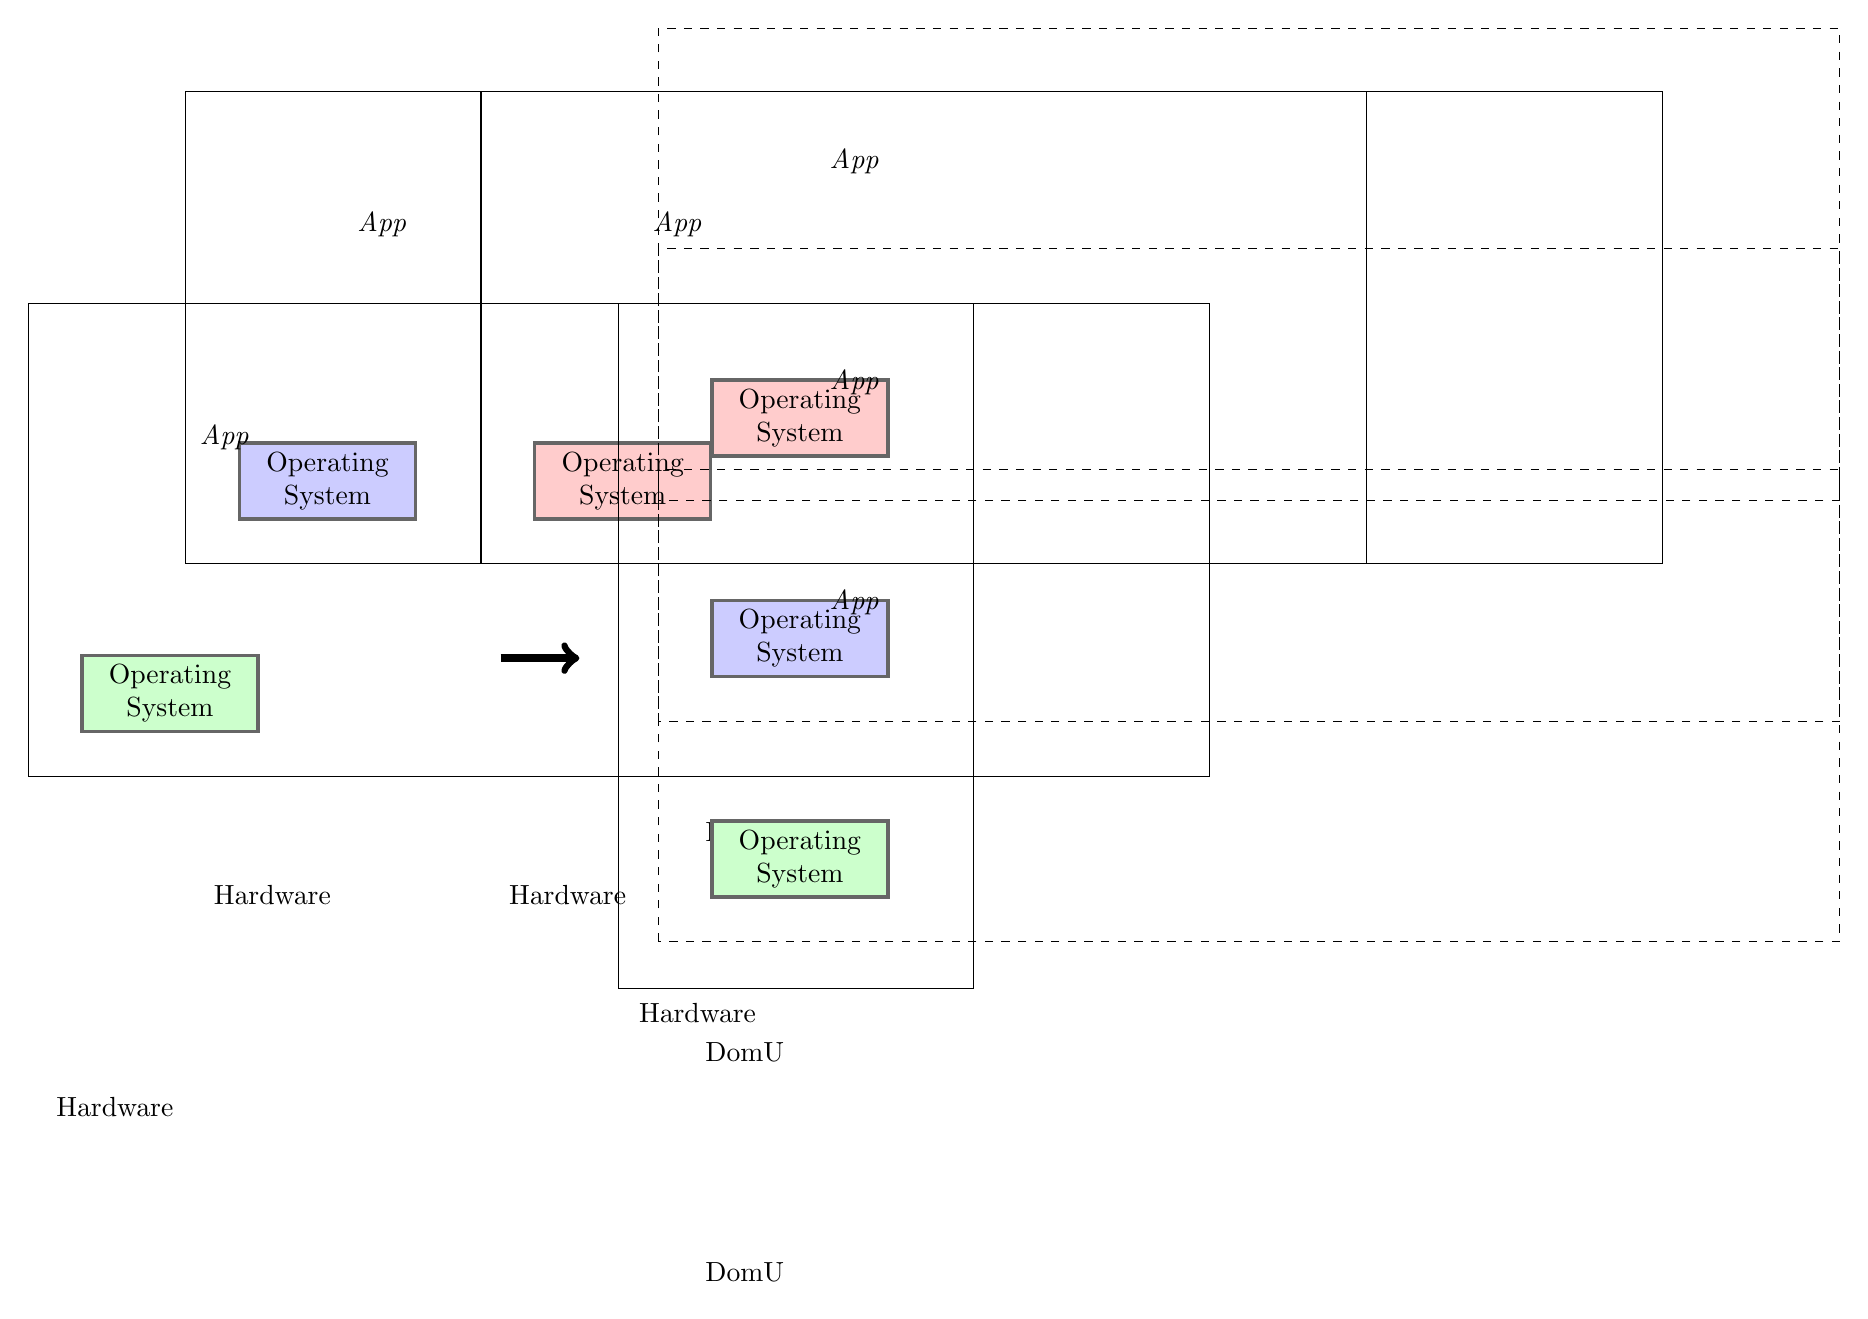
\begin{tikzpicture}[
rednode/.style={rectangle, draw=black!60, fill=red!20, very thick, minimum size=5mm, text width=2cm, text centered},
bluenode/.style={rectangle, draw=black!60, fill=blue!20, very thick, minimum size=5mm, text width=2cm, text centered},
greennode/.style={rectangle, draw=black!60, fill=green!20, very thick, minimum size=5mm, text width=2cm, text centered},]
  % Dialectics
  \draw[black] (\xr, \yr)rectangle(\xr + \xout, \yr + \yout);
  \node[rednode, label={[xshift = \xhard cm, yshift=-\yout cm]Hardware}] at (\xr + \xin, \yr + \yin) {Operating System};
  \node at (\xr + \xapp, \yr + \yapp) {\textit{App}};

  \draw[black] (\xb, \yb)rectangle(\xb + \xout, \yb + \yout);
  \node[bluenode, label={[xshift=\xhard cm, yshift=-\yout cm]Hardware}] at (\xb + \xin, \yb + \yin) {Operating System};
  \node at (\xb + \xapp, \yb + \yapp) {\textit{App}};

  \draw[black] (\xg, \yg)rectangle(\xg + \xout, \yg + \yout);
  \node[greennode, label={[xshift=\xhard cm, yshift=-\yout cm]Hardware}] at (\xg + \xin, \yg + \yin) {Operating System};
  \node at (\xg + \xapp, \yg + \yapp) {\textit{App}};
  
  \draw[black] (9.5, -5.2)rectangle(14,3.5);
  \node at (10.5, -5.5) {\text{Hardware}};
  
  \draw[line width=1mm,->] (8,-1) -- (9,-1);
  
  \draw[dashed] (\xrr, \yrr)rectangle(\xrr + \xout, \yrr + \yout);
  \node[rednode, label={[xshift = \xhard cm, yshift=-\yout cm]DomU}] at (\xrr + \xin, \yrr + \yin) {Operating System};
  \node at (\xrr + \xapp, \yrr + \yapp) {\textit{App}};
  
  \draw[dashed] (\xrr, \ybb)rectangle(\xrr + \xout, \ybb + \yout);
  \node[bluenode, label={[xshift = \xhard cm, yshift=-\yout cm]DomU}] at (\xrr + \xin, \ybb + \yin) {Operating System};
  \node at (\xrr + \xapp, \ybb + \yapp) {\textit{App}};
  
  \draw[dashed] (\xrr, \ygg)rectangle(\xrr + \xout, \ygg + \yout);
  \node[greennode, label={[xshift = \xhard cm, yshift=-\yout cm]DomU}] at (\xrr + \xin, \ygg + \yin) {Operating System};
  \node at (\xrr + \xapp, \ygg + \yapp) {\textit{App}};

\end{tikzpicture}

	\caption{Evolution of software deployment from single \ac{OS} to virtualization}
	\label{fig:tovirt}
\end{figure}

Hypervisor is the software that drives this mechanism. It runs directly on the hardware, uses a separate \ac{OS} installation, and resides outside all the guest \ac{VM}s. At the same time, since the hypervisor manages the allocation and usage of all physical resources, it can see the internal state of each \ac{VM}. 

\subsection{Hypervisor types}\label{sub:hyptypes}
Different vendors provide their solutions in virtualization. Generally, hypervisors are separated in two categories: Type-I or bare-metal hypervisors and type-II or hosted hypervisors. Figure~\ref{fig:hyptypes} shows the basic architectural difference between the two types.

\par Type-II hypervisors are applications which require a host \ac{OS} to run on. Typical type-II solutions are VMWare Workstation and Oracle VirtualBox. These hypervisors work like any other application and the \ac{VM}s run on top of them. Although they are simpler to manage for the average user, as well as for simple applications or use as testing environment, type-II hypervisors perform worse than type-I, as explained below. 

\begin{figure}
	\centering
	\def\xout{15}
\def\yout{6}
\def\x{0}
\def\y{0}
\def\xr{7.75}
%\def\yl{1}
\def\xl{0.25}
\def\yl{0.25}
\def\yoffset{0.8}
\def\xsize{70}
\def\ysize{7}
\def\xapp{2.5}
\def\yapp{4.3}
\def\xos{3.2}
\def\yos{2.2}

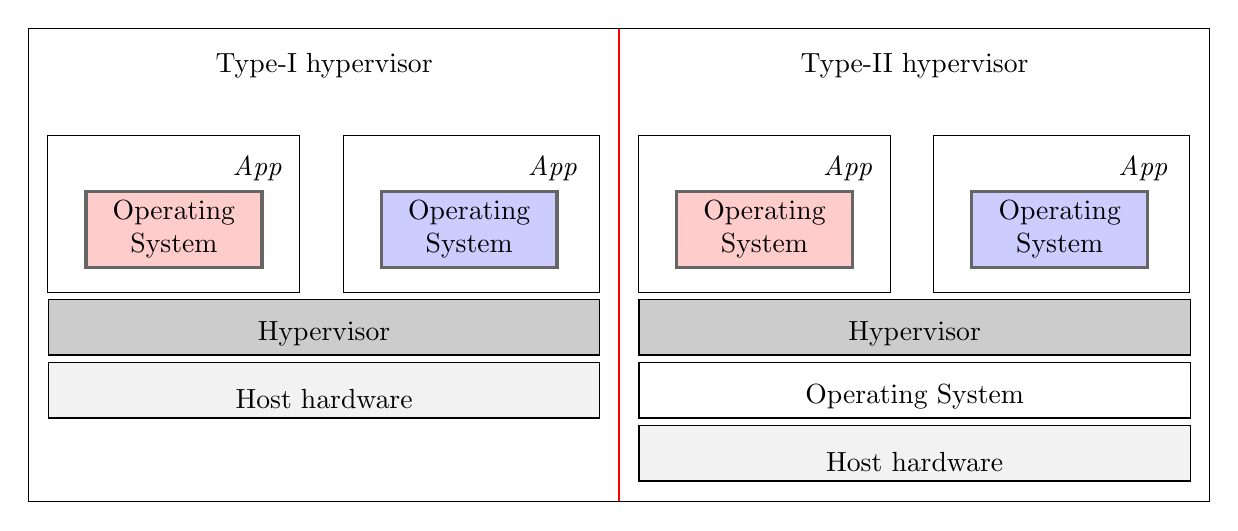
\begin{tikzpicture}[
anode/.style={rectangle, draw=black!60, very thick, minimum size=5mm, minimum width=7cm, minimum height=1cm, text centered},
rednode/.style={rectangle, draw=black!60, fill=red!20, very thick, minimum size=5mm, text width=2cm, text centered},
bluenode/.style={rectangle, draw=black!60, fill=blue!20, very thick, minimum size=5mm, text width=2cm, text centered},]
  
  \draw[black] (\x, \y)rectangle(\xout,\yout);
  \draw[red,thick,-] (7.5, 0) -- (7.5, 6);
  \node (rect) [rectangle, minimum width=\xsize mm, minimum height=\ysize mm, anchor= south west,label={[anchor=south]south:Type-I hypervisor}] at (\xl,\yl+5) {};
  \node (rect) [rectangle, minimum width=\xsize mm, minimum height=\ysize mm, anchor= south west,label={[anchor=south]south:Type-II hypervisor}] at (\xr,\yl+5) {};

  
  \node (rect) [rectangle, draw, fill=black!5, minimum width=\xsize mm, minimum height=\ysize mm, anchor= south west,label={[anchor=south]south:Host hardware}] at (\xl,\yl+\yoffset) {};
  \node (rect) [rectangle, draw, fill=black!20, minimum width=\xsize mm, minimum height=\ysize mm, anchor= south west,label={[anchor=south]south:Hypervisor}] at (\xl,\yl+\yoffset+\yoffset) {};

  \draw[black] (\xl, \yl + \yoffset + \yoffset + \yoffset)rectangle(\xl + \xos, \yl + \yos+ \yoffset + \yoffset + 0.6);
  \node[rednode] at (\xl + \yoffset + \yoffset, \yl + \yoffset + \yoffset + \yoffset + \yoffset) {Operating System};
  \node (rect) [rectangle, minimum width=\xos mm, minimum height=\ysize mm, anchor= south west,label={[anchor=south]south:\textit{App}}] at (\xl+2.5,\yl+3.7) {};

  \draw[black] (4, \yl + \yoffset + \yoffset + \yoffset)rectangle(4.05 + \xos, \yl + \yos+ \yoffset + \yoffset + 0.6);
  \node[bluenode] at (4 + \yoffset + \yoffset, \yl + \yoffset + \yoffset + \yoffset + \yoffset) {Operating System};
  \node (rect) [rectangle, minimum width=\xos mm, minimum height=\ysize mm, anchor= south west,label={[anchor=south]south:\textit{App}}] at (4+2.5,\yl+3.7) {};


  \node (rect) [rectangle, draw, fill=black!5, minimum width=\xsize mm, minimum height=\ysize mm, anchor= south west,label={[anchor=south]south:Host hardware}] at (\xr,\yl) {};
  \node (rect) [rectangle, draw, minimum width=\xsize mm, minimum height=\ysize mm, anchor= south west,label={[anchor=south]south:Operating System}] at (\xr,\yl+\yoffset) {};
  \node (rect) [rectangle, draw, fill=black!20, minimum width=\xsize mm, minimum height=\ysize mm, anchor= south west,label={[anchor=south]south:Hypervisor}] at (\xr,\yl+\yoffset+\yoffset) {};

  \draw[black] (\xr, \yl + \yoffset + \yoffset + \yoffset)rectangle(\xr + \xos, \yl + \yos+ \yoffset + \yoffset + 0.6);
  \node[rednode] at (\xr + \yoffset + \yoffset, \yl + \yoffset + \yoffset + \yoffset + \yoffset) {Operating System};
  \node (rect) [rectangle, minimum width=\xos mm, minimum height=\ysize mm, anchor= south west,label={[anchor=south]south:\textit{App}}] at (\xr+2.5,\yl+3.7) {};

  \draw[black] (\xr + 3.75, \yl + \yoffset + \yoffset + \yoffset)rectangle(\xr + 3.8 + \xos, \yl + \yos+ \yoffset + \yoffset + 0.6);
  \node[bluenode] at (\xr + 3.75 + \yoffset + \yoffset, \yl + \yoffset + \yoffset + \yoffset + \yoffset) {Operating System};
  \node (rect) [rectangle, minimum width=\xos mm, minimum height=\ysize mm, anchor= south west,label={[anchor=south]south:\textit{App}}] at (\xr + 3.75 + 2.5,\yl+3.7) {};
  
\end{tikzpicture}

	\caption{Architectural difference of type-I vs type-II hypervisors}
	\label{fig:hyptypes}
\end{figure}

\par Type-I hypervisors run directly on the hardware, managing the resources directly without the intervention of any host \ac{OS}, providing a significant performance advantage. The advantage comes from eliminating the underlying \ac{OS} of the type-II hypervisors. A Type-II hypervisor must ask the host \ac{OS} for the resources the hypervisor needs to allocate every time, an action that produces performance overhead. Type-I hypervisors implement the resource management on their own since they run on a more privileged \ac{OS} and they are actually part of it. The type-I hypervisors run and at the same privilege level with the \ac{OS} and can manage the resources without asking the host \ac{OS}. Therefore, type-I hypervisors provide a more efficient resource management of the hypervisor and its hosted \ac{VM}s. Type-I hypervisors are most commonly used in server deployment and enterprise solutions, where performance and efficiency are important. 

\subsection{The Xen project}\label{sub:xen}
The product of the Xen project~\cite{xen} is an open-source type-I hypervisor. Its small footprint and limited interface to the guest makes it more robust and secure. The hypervisor runs directly on top of the hardware, as depicted in Figure~\ref{img:xen}. It requires a host \ac{OS} which acts as an interface between the hypervisor and the user, as well as paravirtualized guests. This host \ac{OS} is called control or privileged domain, also known as Dom0, and runs at a more privileged level than the rest of the \ac{VM}s. The rest of the \ac{VM}s run on a lower privilege level and are called guest domains or DomUs. 

\begin{figure}
	\centering
	\begin{tikzpicture}[
rednode/.style={rectangle, draw=black!60, fill=red!20, very thick, minimum size=15mm, text width=2cm, text centered},
bluenode/.style={rectangle, draw=black!60, fill=blue!20, very thick, minimum size=15mm, text width=2cm, text centered},
greennode/.style={rectangle, draw=black!60, fill=green!20, very thick, minimum size=15mm, text width=2cm, text centered},
greynode/.style={rectangle, draw=black!60, fill=black!20, very thick, minimum size=15mm, text width=2cm, text centered},]

\node (rect) [copy shadow={draw=black!10, fill=black!40, opacity=0.5}, fill=green!20, rectangle, draw=black!70, minimum width=150mm, minimum height=10mm, anchor= south west,
	label={[anchor=south, yshift=0.15cm, xshift=-6.5cm]south:I/O}, 
	label={[anchor=south, yshift=0.15cm, xshift=-1.5cm]south:Memory}, 
	label={[anchor=south, yshift=0.15cm, xshift=1.5cm]south:\ac{CPU}}, 
	label={[anchor=south, yshift=0.15cm, xshift=6.5cm]south:\textbf{HW}}] 
at (0, 0) {};

\node (rect) [copy shadow={draw=black!10, fill=black!40, opacity=0.5}, fill=blue!15, rectangle, draw=black!70, minimum width=150mm, minimum height=10mm, anchor= south west,
	label={[anchor=south, yshift=0.15cm, xshift=-4.5cm]south:Config}, 
	label={[anchor=south, yshift=0.15cm, xshift=-2cm]south:Scheduler}, 
	label={[anchor=south, yshift=0.15cm, xshift=0cm]south:MMU}, 
	label={[anchor=south, yshift=0.15cm, xshift=2cm]south:Timers},
	label={[anchor=south, yshift=0.15cm, xshift=4.5cm]south:Interrupts},
	label={[anchor=south, yshift=0.15cm, xshift=6.5cm]south:\textbf{XEN}}] 
at (0, 1.5) {};

\draw[copy shadow={draw=black!10, fill=black!40, opacity=0.5}, black, fill=white] (0, 6.5)rectangle(2, 8.5);
\draw[black, fill = black!80] (0.2, 6.7)rectangle(1.8, 8);
\node[anchor= south west] at (0, 7.9) {\textit{Console}};

\draw[copy shadow={draw=black!10, fill=black!40, opacity=0.5}, black, fill=white] (0, 3)rectangle(3, 6);
\node[anchor= south west, greynode, label={}] at (0.3, 3.25) {Dom0 Kernel};
\node[anchor= south west] at (0, 5.25) {\textit{VM0 or Dom0}};



\draw[copy shadow={draw=black!10, fill=black!40, opacity=0.5}, black, fill=white] (12, 3)rectangle(15, 6);
\node[anchor= south west, greennode, label={}] at (12.3, 3.25) {Guest OS};
\node[anchor= south west] at (12, 5.25) {\textit{VMn}};

\draw[anchor= south west, draw=green!70, line width=1mm,<->] (2.6,3.7) -- (12.3,3.7);

\draw[copy shadow={draw=black!10, fill=black!40, opacity=0.5}, black, fill=white] (8.5, 3)rectangle(11.5, 6);
\node[anchor= south west, bluenode, label={}] at (8.8, 3.25) {Guest OS};
\node[anchor= south west] at (8.5, 5.25) {\textit{VM2}};

\draw[anchor= south west, draw=blue!70, line width=1mm,<->] (2.6,4) -- (8.8,4);


\draw[copy shadow={draw=black!10, fill=black!40, opacity=0.5}, black, fill=white] (5, 3)rectangle(8, 6);
\node[anchor= south west, rednode, label={}] at (5.3, 3.25) {Guest OS};
\node[anchor= south west] at (5, 5.25) {\textit{VM1}};


\draw[anchor= south west, draw=red!70, line width=1mm,<->] (2.6,4.3) -- (5.3,4.3);

\draw[anchor= south west, draw=orange, line width=1mm,<->] (1.05,0.8) -- (1.05,3.25);
\draw[anchor= south west, draw=orange, line width=1mm,<->] (1.05,4.8) -- (1.05,6.5);

\end{tikzpicture}
	\caption{Xen Hypervisor Architecture}
	\label{img:xen}
\end{figure}

\par To understand how this happens, we need to introduce another \ac{CPU} architectural feature, which provides different privilege levels for the execution of the \ac{CPU} instructions, depending on the nature of the program invoking them. This mechanism called protection rings, is present on all modern \ac{CPU}s and is used by all modern \acp{OS}. Protection rings are numbered 0 to 3, with 0 being the most privileged. Usually, applications run in ring 3, also called user mode, and the kernel and device drivers run in ring 0, also called privileged or supervisor mode. But, in order to allocate and manage the shared resources the hypervisor must run at a more privileged level than the guest \ac{OS}, otherwise there is a conflict when the guest \ac{OS} and the hypervisor try to manage a same resource. Initially, paravirtualization, a technique where \ac{OS} vendors had to modify their kernels to run on a different privilege level, besides 0, like 1 or 2, was used to avoid that conflict between the guest \ac{OS} kernel and the hypervisor.

\par For type-I hypervisors to work more efficiently and without any guest \ac{OS} modification, \ac{CPU} manufacturers have introduced a new ring -1 to support virtualization. The new ring, called hypervisor mode, is even more privileged than ring 0 and is employed only during hypervisor execution. This architecture is supported on newer \ac{CPU}s that employ \ac{VT}, VT-x for Intel and AMD-V for AMD processors. 

As virtualization keeps advancing, there is always the question of whether we can leverage virtualization to provide more than efficient sharing and usage of resources. The unique ability of the hypervisor to access the state of a \ac{VM}, at the fine grain level of \ac{CPU} registers and memory bytes, has been the center of research ever since the technology was invented. 

\begin{figure}
	\centering
	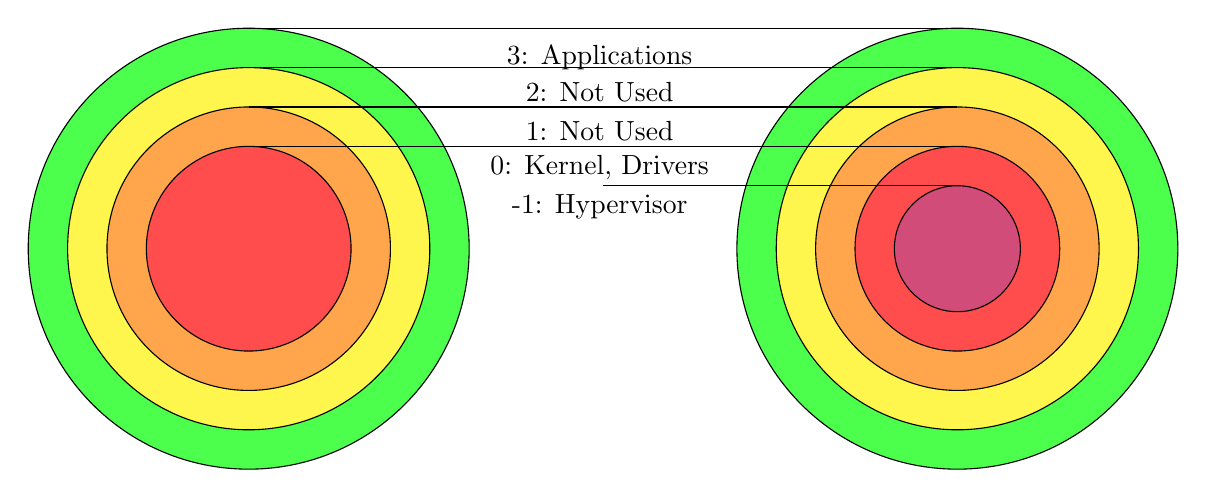
\begin{tikzpicture}[
rednode/.style={circle, draw=red!60, fill=red!30, very thick, minimum size=5mm, text width=2cm, text centered},
bluenode/.style={rectangle, draw=black!60, fill=blue!20, very thick, minimum size=5mm, text width=2cm, text centered},]
  
  	\filldraw[fill=green!70, draw=black] (0, 0) circle (2.8cm);
  	\filldraw[fill=yellow!70, draw=black] (0, 0) circle (2.3cm);
	\filldraw[fill=orange!70, draw=black] (0, 0) circle (1.8cm);
	\filldraw[fill=red!70, draw=black] (0, 0) circle (1.3cm);


  	\filldraw[fill=green!70, draw=black] (9, 0) circle (2.8cm);
	\filldraw[fill=yellow!70, draw=black] (9, 0) circle (2.3cm);
	\filldraw[fill=orange!70, draw=black] (9, 0) circle (1.8cm);
	\filldraw[fill=red!70, draw=black] (9, 0) circle (1.3cm);
	\filldraw[fill=purple!70, draw=black] (9, 0) circle (0.8cm);
	
	\draw[black, -] (0, 2.8) -- (9, 2.8);
	\draw[black, -] (0, 2.3) -- (9, 2.3);
	\draw[black, -] (0, 1.8) -- (9, 1.8);
	\draw[black, -] (0, 1.3) -- (9, 1.3);
	\draw[black, -] (4.5, 0.8) -- (9, 0.8);

	\node (rect) [rectangle, minimum width=30mm, minimum height=4mm, anchor= south west,label={[anchor=south]south:3: Applications}] at (2.95, 2.15) {};
	\node (rect) [rectangle, minimum width=30mm, minimum height=4mm, anchor= south west,label={[anchor=south]south:2: Not Used}] at (2.95, 1.75) {};
	\node (rect) [rectangle, minimum width=30mm, minimum height=4mm, anchor= south west,label={[anchor=south]south:1: Not Used}] at (2.95, 1.25) {};
	\node (rect) [rectangle, minimum width=30mm, minimum height=4mm, anchor= south west,label={[anchor=south]south:0: Kernel, Drivers}] at (2.95, 0.75) {};	
	\node (rect) [rectangle, minimum width=30mm, minimum height=4mm, anchor= south west,label={[anchor=south]south:-1: Hypervisor}] at (2.95, 0.25) {};	
		
\end{tikzpicture}
	\caption{x86 protection rings}
	\label{fig:rings}
\end{figure}

\section{Virtual Machine Introspection}\label{sec:vmi}
In this section we introduce a rough timeline of the \acp{API}, significant for our research, that were evolved around virtualization and \ac{VMI}. These include \emph{LibVMI} and the later implemented \emph{altp2m} for Xen. We mention \emph{DRAKVUF}~\cite{lengyel2014drakvuf}, a tool that employs LibVMI and altp2m to implement a virtualization based agentless black-box binary analysis system. DRAKVUF is the platform we based our solution on. 	

\par First introduced as a concept by Garfinkel et al~\cite{garfinkel2003virtual}, \ac{VMI} leverages the more privileged status of the hypervisor to inspect the internal state of a \ac{VM}. The Xen hypervisor was first to include introspection methods to inspect its guest \ac{VM}s. Although these introspection methods where included in Xen, implementing introspection in a way that is secure and efficient was a non-trivial task. To make these methods more accessible to programmers, XenAccess~\cite{payne2007secure} was implemented, as well as an \ac{API} called \emph{mem-events}. Because of strong research and security interest, introspection in Xen progressed and eventually LibVMI~\cite{payne2011libvmi}, a library that makes the implementation and automation of introspection on the Xen hypervisor easier, was introduced. LibVMI provides access to part of the hypervisors introspection methods to third-party applications, using a C or Python interface, the later called PyVMI. 

\par Initially, hypervisor memory management included an extra step in the memory access mechanism, because each \ac{VM} assumes that it has complete control over the entire address space, and assumes that it writes directly on the hardware. Normally the \ac{OS} would translate the virtual address used by an application to a physical address on the hardware. To a hypervisor, each \ac{VM} is essentially an application. Since every \ac{OS} will eventually try to write on the same physical address, the hypervisor must make a distinction between the \ac{VM}s. To achieve that distinction the hypervisor assigns each \ac{VM} a specific physical address space and tracks the overall memory usage with an additional \ac{PT} translating between a \ac{VM} specific \ac{GMFN} and the \ac{MFN}, as explained in Chisnall~\cite{chisnall2008definitive}.

\begin{figure}
	\centering
	\begin{tikzpicture}[
rednode/.style={circle, draw=red!60, fill=red!30, very thick, minimum size=5mm, text width=2cm, text centered},
bluenode/.style={rectangle, draw=black!60, fill=blue!20, very thick, minimum size=5mm, text width=2cm, text centered},]
 
   	\node (rect) [copy shadow={draw=black!20, fill=black!40, opacity=0.5}, fill=white, rectangle, draw=black!50, minimum width=5mm, minimum height=5mm, anchor= south west,label={}] at (0, 5) {};
   	\node (rect) [copy shadow={draw=black!20, fill=black!40, opacity=0.5}, fill=white, rectangle, draw=black!50, minimum width=5mm, minimum height=5mm, anchor= south west,label={}] at (0.5, 5) {};
   	\node (rect) [copy shadow={draw=black!20, fill=black!40, opacity=0.5}, fill=red!60, rectangle, draw=black!50, minimum width=5mm, minimum height=5mm, anchor= south west,label={}] at (1, 5) {};
   	\node (rect) [copy shadow={draw=black!20, fill=black!40, opacity=0.5}, fill=blue!60, rectangle, draw=black!50, minimum width=5mm, minimum height=5mm, anchor= south west,label={}] at (1.5, 5) {};
   	\node (rect) [copy shadow={draw=black!20, fill=black!40, opacity=0.5}, fill=green!60, rectangle, draw=black!50, minimum width=5mm, minimum height=5mm, anchor= south west,label={}] at (2, 5) {};
   	\node (rect) [copy shadow={draw=black!20, fill=black!40, opacity=0.5}, fill=white, rectangle, draw=black!50, minimum width=5mm, minimum height=5mm, anchor= south west,label={}] at (2.5, 5) {};
   	\node (rect) [copy shadow={draw=black!20, fill=black!40, opacity=0.5}, fill=white, rectangle, draw=black!50, minimum width=5mm, minimum height=5mm, anchor= south west,label={}] at (3, 5) {};
   	\node (rect) [copy shadow={draw=black!20, fill=black!40, opacity=0.5}, fill=white, rectangle, draw=black!50, minimum width=5mm, minimum height=5mm, anchor= south west,label={}] at (3.5, 5) {};
   	
   	\node (rect) [copy shadow={draw=black!20, fill=black!40, opacity=0.5}, fill=green!60, rectangle, draw=black!50, minimum width=5mm, minimum height=5mm, anchor= south west,label={}] at (0, 2.5) {};
	\node (rect) [copy shadow={draw=black!20, fill=black!40, opacity=0.5}, fill=white, rectangle, draw=black!50, minimum width=5mm, minimum height=5mm, anchor= south west,label={}] at (0.5, 2.5) {};
	\node (rect) [copy shadow={draw=black!20, fill=black!40, opacity=0.5}, fill=white, rectangle, draw=black!50, minimum width=5mm, minimum height=5mm, anchor= south west,label={}] at (1, 2.5) {};
	\node (rect) [copy shadow={draw=black!20, fill=black!40, opacity=0.5}, fill=white, rectangle, draw=black!50, minimum width=5mm, minimum height=5mm, anchor= south west,label={}] at (1.5, 2.5) {};
	\node (rect) [copy shadow={draw=black!20, fill=black!40, opacity=0.5}, fill=white, rectangle, draw=black!50, minimum width=5mm, minimum height=5mm, anchor= south west,label={}] at (2, 2.5) {};
	\node (rect) [copy shadow={draw=black!20, fill=black!40, opacity=0.5}, fill=blue!60, rectangle, draw=black!50, minimum width=5mm, minimum height=5mm, anchor= south west,label={}] at (2.5, 2.5) {};
	\node (rect) [copy shadow={draw=black!20, fill=black!40, opacity=0.5}, fill=white, rectangle, draw=black!50, minimum width=5mm, minimum height=5mm, anchor= south west,label={}] at (3, 2.5) {};
	\node (rect) [copy shadow={draw=black!20, fill=black!40, opacity=0.5}, fill=red!60, rectangle, draw=black!50, minimum width=5mm, minimum height=5mm, anchor= south west,label={}] at (3.5, 2.5) {};
	
   	\node (rect) [copy shadow={draw=black!20, fill=black!40, opacity=0.5}, fill=white, rectangle, draw=black!50, minimum width=5mm, minimum height=5mm, anchor= south west,label={}] at (0, 0) {};
	\node (rect) [copy shadow={draw=black!20, fill=black!40, opacity=0.5}, fill=blue!60, rectangle, draw=black!50, minimum width=5mm, minimum height=5mm, anchor= south west,label={}] at (0.5, 0) {};
	\node (rect) [copy shadow={draw=black!20, fill=black!40, opacity=0.5}, fill=white, rectangle, draw=black!50, minimum width=5mm, minimum height=5mm, anchor= south west,label={}] at (1, 0) {};
	\node (rect) [copy shadow={draw=black!20, fill=black!40, opacity=0.5}, fill=green!60, rectangle, draw=black!50, minimum width=5mm, minimum height=5mm, anchor= south west,label={}] at (1.5, 0) {};
	\node (rect) [copy shadow={draw=black!20, fill=black!40, opacity=0.5}, fill=white, rectangle, draw=black!50, minimum width=5mm, minimum height=5mm, anchor= south west,label={}] at (2, 0) {};
	\node (rect) [copy shadow={draw=black!20, fill=black!40, opacity=0.5}, fill=red!60, rectangle, draw=black!50, minimum width=5mm, minimum height=5mm, anchor= south west,label={}] at (2.5, 0) {};
	\node (rect) [copy shadow={draw=black!20, fill=black!40, opacity=0.5}, fill=white, rectangle, draw=black!50, minimum width=5mm, minimum height=5mm, anchor= south west,label={}] at (3, 0) {};
	\node (rect) [copy shadow={draw=black!20, fill=black!40, opacity=0.5}, fill=white, rectangle, draw=black!50, minimum width=5mm, minimum height=5mm, anchor= south west,label={}] at (3.5, 0) {};
	
   	\node (rect) [rectangle, minimum width=30mm, minimum height=4mm, anchor= south west,label={[anchor=south]south:Application}] at (-3, 5) {};
	\node (rect) [rectangle, minimum width=30mm, minimum height=4mm, anchor= south west,label={[anchor=south]south:Virtual}] at (4.5, 5) {};
	\node (rect) [rectangle, minimum width=30mm, minimum height=4mm, anchor= south west,label={[anchor=south]south:Kernel}] at (-3, 2.5) {};
	\node (rect) [rectangle, minimum width=30mm, minimum height=4mm, anchor= south west,label={[anchor=south]south:Pseudo-physical}] at (4.5, 2.5) {};
	\node (rect) [rectangle, minimum width=30mm, minimum height=4mm, anchor= south west,label={[anchor=south]south:Hypervisor}] at (-3, 0) {};
	\node (rect) [rectangle, minimum width=30mm, minimum height=4mm, anchor= south west,label={[anchor=south]south:Machine}] at (4.5, 0) {};
	
	\draw[line width=0.3mm, red!80, ->] (1.25, 5) -- (3.75, 3);
	\draw[line width=0.3mm, blue!80, ->] (1.75, 5) -- (2.75, 3);
	\draw[line width=0.3mm, green!80, ->] (2.25, 5) -- (0.25, 3);

	\draw[line width=0.3mm, green!80, ->] (0.25, 2.5) -- (1.75, 0.5);
	\draw[line width=0.3mm, blue!80, ->] (2.75, 2.5) -- (0.75, 0.5);
	\draw[line width=0.3mm, red!80, ->] (3.75, 2.5) -- (2.75, 0.5);

		
\end{tikzpicture}
	\caption{Hypervisor memory management concept}
	\label{fig:hypmm}
\end{figure}

\par With the introduction of \ac{IOMMU}, this extra step is no longer needed, because hardware \acp{EPT} were included in the \ac{CPU}s and the hypervisors can use these hardware \acp{EPT} instead of software ones, a method called \ac{HAP}. \ac{HAP} implemented better isolation, and therefore enhanced security between the \acp{VM}, while at the same time the overhead reduced significantly. Following that development, as well as Intel's addition of 512 \acp{EPT} in its Haswell generation \ac{CPU}, XenAccess and mem-events were redesigned and were evolved to a system called \emph{altp2m}. One of the most critical changes that came with altp2m was the concurrent assignment of multiple \ac{EPT}s per \ac{VM} (Fig.~\ref{fig:ept}). Additionally, monitoring processes of multi-virtual\ac{CPU} guests is more secure, because each virtual \ac{CPU} can be assigned its own \ac{EPT}. This was a significant improvement, as the hypervisor can keep track of different \acp{EPT} with different permissions, which can change during the execution of the \ac{VM}. Other solutions keep only one \ac{EPT} per \ac{VM}, resulting in a less secure and isolated virtual environment between the \acp{VM} and the \acp{VM}' processes.

\begin{figure}[ht]
	\centering
	\scalebox{0.95}{\begin{tikzpicture}[
rednode/.style={circle, draw=red!60, fill=red!30, very thick, minimum size=5mm, text width=2cm, text centered},
bluenode/.style={rectangle, draw=black!60, fill=blue!20, very thick, minimum size=5mm, text width=2cm, text centered},]
   	
   	\node (rect) [copy shadow={draw=black!10, fill=black!40, opacity=0.5}, fill=white, rectangle, draw=black!70, minimum width=50mm, minimum height=70mm, anchor= south west,label={}] at (0, 0) {};
	\node (rect) [fill=white, rectangle, draw=black!70, minimum width=50mm, minimum height=10mm, anchor= south west,label={[anchor=south]center:VM}] at (0, 0) {};


	\node (rect) [fill=blue!30, rectangle, draw=black!70, minimum width=50mm, minimum height=20mm, anchor= south west,label={[anchor=south]center:Guest Physical Address}] at (0, 1) {};
	\node (rect) [fill=white, rectangle, draw=black!70, text width=4cm, minimum width=46mm, minimum height=10mm, anchor= south west,label={[anchor=south, yshift=-0.2cm]south:\begin{tabular}{c}
		Process 1: Guest Virtual \\ Address (GVA)
		\end{tabular}}] at (0.2, 5.9) {};
	\node (rect) [fill=white, rectangle, draw=black!70, text width=4cm, minimum width=46mm, minimum height=7mm, anchor= south west,label={[anchor=south]south:Process 2: (GVA) }] at (0.2, 5) {};
	\node (rect) [fill=white, rectangle, draw=black!70, text width=4cm, minimum width=46mm, minimum height=7mm, anchor= south west,label={[anchor=south]south:Process 3: (GVA) }] at (0.2, 4.1) {};
	\node (rect) [fill=white, rectangle, draw=black!70, text width=4cm, minimum width=46mm, minimum height=7mm, anchor= south west,label={[anchor=south]south:Process n: (GVA) }] at (0.2, 3.2) {};
	\node (rect) [copy shadow={draw=black!10, fill=black!40, opacity=0.5}, fill=green!20, rectangle, draw=black!70, minimum width=50mm, minimum height=10mm, anchor= south west,label={[anchor=south]south:Machine Physical Address}] at (0, -1.2) {};
		
	\draw[->, line width=2pt] (5.2, 5) arc[x radius=-1cm, y radius=-1.3cm, start angle=270, end angle=90];
	\draw[->, line width=2pt] (5.2, 1.5) arc[x radius=-1cm, y radius=-1.1cm, start angle=270, end angle=90];



   	\node (rect) [copy shadow={draw=black!10, fill=black!40, opacity=0.5}, fill=white, rectangle, draw=black!70, minimum width=50mm, minimum height=70mm, anchor= south west,label={}] at (7, 0) {};
	\node (rect) [fill=white, rectangle, draw=black!70, minimum width=50mm, minimum height=10mm, anchor= south west,label={[anchor=south]center:VM}] at (7, 0) {};
	\node (rect) [fill=blue!30, rectangle, draw=black!70, minimum width=50mm, minimum height=20mm, anchor= south west,label={[anchor=south]center:Guest Physical Address}] at (7, 1) {};
	\node (rect) [fill=white, rectangle, draw=black!70, text width=4cm, minimum width=46mm, minimum height=10mm, anchor= south west,label={[anchor=south, yshift=-0.2cm]south:\begin{tabular}{c}
	Process 1: Guest Virtual \\ Address (GVA)
	\end{tabular}}] at (7.2, 5.9) {};
	\node (rect) [fill=white, rectangle, draw=black!70, text width=4cm, minimum width=46mm, minimum height=7mm, anchor= south west,label={[anchor=south]south:Process 2: (GVA) }] at (7.2, 5) {};
	\node (rect) [fill=white, rectangle, draw=black!70, text width=4cm, minimum width=46mm, minimum height=7mm, anchor= south west,label={[anchor=south]south:Process 3: (GVA) }] at (7.2, 4.1) {};
	\node (rect) [fill=white, rectangle, draw=black!70, text width=4cm, minimum width=46mm, minimum height=7mm, anchor= south west,label={[anchor=south]south:Process n: (GVA) }] at (7.2, 3.2) {};
	\node (rect) [copy shadow={draw=black!10, fill=black!40, opacity=0.5}, fill=green!20, rectangle, draw=black!70, minimum width=50mm, minimum height=10mm, anchor= south west,label={[anchor=south]south:Machine Physical Address}] at (7, -1.2) {};

	\draw[->, line width=2pt] (12.2, 5) arc[x radius=-1cm, y radius=-1.3cm, start angle=270, end angle=90];
	\draw[->, line width=2pt, draw=black!50] (12.2, 1.45) arc[x radius=-1cm, y radius=-1.25cm, start angle=270, end angle=90];
	\draw[->, line width=2pt, draw=black!65] (12.2, 1.6) arc[x radius=-1cm, y radius=-1.2cm, start angle=270, end angle=90];
	\draw[->, line width=2pt, draw=black!80] (12.2, 1.75) arc[x radius=-1cm, y radius=-1.15cm, start angle=270, end angle=90];
	\draw[->, line width=2pt, draw=black] (12.2, 1.9) arc[x radius=-1cm, y radius=-1.1cm, start angle=270, end angle=90];
			
\end{tikzpicture}}
	\caption{Normal vs altp2m multiple \ac{EPT} assignment}
	\label{fig:ept}
\end{figure}

\par LibVMI, as mentioned earlier, is an \ac{API} which provides exposure to a subset of Xen’s \ac{VMI} functionalities, as well as other platforms. LibVMI makes it possible to monitor the state of any \ac{VM}, including memory and \ac{CPU} state. Memory can be accessed directly, using physical addresses, or indirectly with the use of virtual addresses, \ac{OS} symbols, and user application symbols. It can monitor memory and register events, like memory read, memory write, register value change, and provide notifications for them, allowing this way the execution of callback functions, while the monitoring application resides outside the \acp{VM} and accesses the \acp{VM} through the hypervisor (Fig.~\ref{fig:libvmi}). 


\begin{figure}[ht]
	\centering
	\begin{tikzpicture}[
rednode/.style={circle, draw=red!60, fill=red!30, very thick, minimum size=5mm, text width=2cm, text centered},
bluenode/.style={rectangle, draw=black!60, fill=blue!20, very thick, minimum size=5mm, text width=2cm, text centered},]
  
   	\node (rect) [copy shadow={draw=black!10, fill=black!40, opacity=0.5}, fill=blue!10, rectangle, rounded corners, draw=black, minimum width=50mm, minimum height=50mm, label={[yshift=-1.5cm]north:\begin{tabular}{c}
   		LibVMI System \\ (Host OS/Privileged \ac{VM})
   		\end{tabular}}] at (0, -1) {};
	\node (rect) [fill=green!10, rectangle, draw=black!80, minimum width=45mm, minimum height=10mm, label={[yshift=-0.8cm]LibVMI}] at (0, -2.5) {}; 
	\node (rect) [fill=green!10, rectangle, draw=black!80, minimum width=20mm, minimum height=10mm, label={[yshift=-0.9cm]App(C)}] at (-1.25, -1.3) {}; 
	\node (rect) [fill=green!10, rectangle, draw=black!80, minimum width=20mm, minimum height=10mm, label={[yshift=-0.9cm]PyVMI}] at (1.2, -1.3) {}; 

   	\node (rect) [copy shadow={draw=black!10, fill=black!40, opacity=0.5}, fill=blue!10, rectangle, rounded corners, draw=black, minimum width=50mm, minimum height=50mm, label={}] at (6.6, -1) {};
   	\node (rect) [copy shadow={draw=black!10, fill=black!40, opacity=0.5}, fill=blue!10, rectangle, rounded corners, draw=black, minimum width=50mm, minimum height=50mm, label={}] at (6.3, -1.3) {};
   	\node (rect) [copy shadow={draw=black!10, fill=black!40, opacity=0.5}, fill=blue!10, rectangle, rounded corners, draw=black, minimum width=50mm, minimum height=50mm, label={[yshift=-1cm]north:Monitored \ac{VM}s}] at (6, -1.6) {};
   	
   	\node (rect) [fill=blue!10, rectangle, minimum width=20mm, minimum height=10mm, label={[yshift=-2.5cm]\begin{tabular}{c}
   		Windows \\ Linux \\ Other \ac{OS}
   		\end{tabular}}] at (6, -1) {}; 

   	\node (rect) [copy shadow={draw=black!10, fill=black!40, opacity=0.5}, fill=blue!10, rectangle, rounded corners, draw=black, minimum width=100mm, minimum height=10mm, label={[yshift=-0.9cm]north:Hypervisor/Virtualization}] at (3, -7) {};

	\draw[->, line width=2pt, draw=black] (3, -6.5) arc[x radius=6cm, y radius=-3.5cm, start angle=120, end angle=180];
	\draw[->, line width=2pt, draw=black] (3, -6.5) arc[x radius=-6cm, y radius=-2.8cm, start angle=120, end angle=180];
\end{tikzpicture}
	\caption{LibVMI out of guest access of \ac{VM} state}
	\label{fig:libvmi}
\end{figure}

\par LibVMI focuses in a subset of introspection methods that provide memory reading and writing capabilities from running \ac{VM}s. It also provides methods for accessing and modifying \ac{CPU} registers, as well as helper methods to pause and unpause a \ac{VM}. Accessing a \ac{VM}'s memory space is not a trivial task. After detecting where the page directory is, a scan of the page tables follows to detect the memory mapping of the running process. This gets translated to a virtual address, which later, the hypervisor translates to a physical address. Figure~\ref{fig:accesskernel} shows a slightly different request, that of reading a kernel symbol.

\par Xen’s introspection methods significantly impact system security. The monitoring application resides on the host and accesses the \ac{VM}s' state from the hypervisor, which implies a zero-footprint monitoring tool from the \ac{VM}'s perspective. The monitor does not leave a trace of its action that can be detected from inside the guest.

\begin{figure}[ht]
	\centering
	\begin{tikzpicture}[
rednode/.style={circle, draw=red!60, fill=red!30, very thick, minimum size=5mm, text width=2cm, text centered},
bluenode/.style={rectangle, draw=black!60, fill=blue!20, very thick, minimum size=5mm, text width=2cm, text centered},]

  
   	\node[anchor= south west, copy shadow={draw=black!10, fill=black!40, opacity=0.5}, fill=white, rectangle, rounded corners, draw=black, minimum width=50mm, minimum height=70mm, label={[yshift=-1cm]north:Dom0}] at (0, 0) {};
   	
	\node[anchor= south west, fill=white, rectangle, draw=black!80, rounded corners, minimum width=45mm, minimum height=10mm, label={[yshift=-0.8cm]VMI Application}] at (0.25, 5) {}; 
	\node (rect) [anchor= south west, fill=white, rectangle, draw=black!80, rounded corners, minimum width=45mm, minimum height=10mm, label={[yshift=-0.8cm]LibVMI}] at (0.25, 3.5) {}; 
	
	\node[dashed, anchor= south west, fill=white, rectangle, draw=black!80, minimum width=20mm, minimum height=15mm, label={[yshift=-1.5cm]\begin{tabular}{c}
		System \\ Map
		\end{tabular}}] at (2.5, 1.5) {}; 
	
   	\node[anchor= south west, copy shadow={draw=black!10, fill=black!40, opacity=0.5}, fill=white, rectangle, rounded corners, draw=black, minimum width=75mm, minimum height=42mm, label={[yshift=-0.7cm]north:User VM (DomU)}] at (7, 0) {};

	\node[dashed, anchor= south west, fill=white, rectangle, draw=black!80, minimum width=20mm, minimum height=20mm, label={[yshift=-1.7cm]\begin{tabular}{c}
		Page \\ Directory
		\end{tabular}}] at (7.2, 1.5) {}; 

	\node[dashed, anchor= south west, fill=white, rectangle, draw=black!80, minimum width=20mm, minimum height=20mm, label={[yshift=-1.7cm]\begin{tabular}{c}
	Page \\ Table
	\end{tabular}}] at (9.6, 1.5) {}; 

	\node[dashed, anchor= south west, fill=white, rectangle, draw=black!80, minimum width=20mm, minimum height=20mm, label={[yshift=-1.7cm]\begin{tabular}{c}
	Kernel \\ Data
	\end{tabular}}] at (12.2, 0.5) {}; 

	\draw[anchor= south west, draw=red!70, line width=1mm,->] (4, 5) -- (4, 4.5);
	\draw[anchor= south west, draw=red!70, line width=1mm,->] (4, 3.5) -- (4, 3);
	
	\draw[anchor= south west, draw=red!70, line width=1mm,->] (4.5, 2) -- (7.2, 2);
	\draw[anchor= south west, draw=red!70, line width=1mm,->] (9.2, 2) -- (9.6, 2);
	\draw[anchor= south west, draw=red!70, line width=1mm,->] (11.6, 2) -- (12.2, 2);
	
	\draw[anchor= south west, draw=blue!60, line width=1mm,->] (12.2, 1) -- (1, 1) -- (1, 3.5);
	\draw[anchor= south west, draw=blue!60, line width=1mm,->] (1, 4.5) -- (1, 5);

	\node[anchor= south west, rectangle, text width=90mm, label={}, font=\small] at (5.5, 4.5) {\textit{
		The VMI application requests a kernel symbol. 
		LibVMI looks up the symbol in the System Map.
		Then it looksup in the Page Directory to find the correct Page Table.
		It finds the symbol in the Page Table, reads the data and returns the value to the application.}};


\end{tikzpicture}
%	\includegraphics{libvmi}
	\caption{Using LibVMI to access the value of a kernel symbol}
	\label{fig:accesskernel}
\end{figure}

\par Although this development was game-changing, it had its drawbacks. Just monitoring that values of specific parts of memory, or the \ac{CPU} registers, over a time interval to make any inferences about the running state of the \ac{VM} leaves the \ac{VM} vulnerable during the waiting period. A solution is to trap the memory regions that we want to monitor for access or modification. But this can be detected by a knowledgeable adversary. 

\par To solve this problem, LibVMI, altp2m, along with the substantial number of \ac{EPT}s on the latest \ac{CPU}s, were were combined in DRAKVUF~\cite{lengyel2014drakvuf}, a dynamic malware analysis platform. One of DRAKVUF's most significant key features is that it traps the memory addresses the user wants to monitor for access. When the event gets triggered, the \ac{EPT} with the trapped address gets swapped with the original, so that the execution of the guest \ac{VM} continues. This allows the monitoring of an arbitrary number of memory addresses, providing notification and response capabilities on every such event, while at the same time being untraceable from inside the guest.


\section{System Calls}\label{sec:syscalls}
Modern \ac{OS}s are responsible for allocating their resources efficiently and securely to themselves, as well as to the user level applications. The part of the \ac{OS} assigned to manage these resources, like memory, hard disk drive access, or \ac{CPU} time, is the kernel of the \ac{OS}. The kernel, which runs in its own space, is the heart of the \ac{OS} that makes everything work in harmony without conflicts or resolves them if there are any. When an application is running, it runs in the so-called user-space. This distinction exists to prevent applications from having direct access to the underlying hardware and is enforced with the protection rings, explained previously. The running application has no knowledge of any other application being executed on the same machine, and whenever it requires some resource, it asks the \ac{OS} through the kernel. The kernel, on its behalf, accesses the hard disk drive, allocates memory, or executes other commands that are considered privileged and the application cannot execute. It handles all the low-level details of what the application asked and returns the results of the action. 

\par This very complicated software is the most crucial part of the \ac{OS}. Therefore, not every process can access the kernel directly or invoke all the kernel's functions in order to avoid corruption or misuse the low-level access the kernel has, to gain access where a process should not. This limited interface to the kernel, a sort of protection mechanism, is called a system call. The details of making a system call depend on the \ac{OS}.

\par Programming with a high-level language usually does not involve making system calls directly. Most languages have implemented wrappers for making a system call and simplifying the system call interface. Regardless, the application will eventually have to make a system call to access some of the system's resources. Files is one type of resource an application needs to request access from the \ac{OS}. This is performed with the \emph{open} system call. Access to input devices, like a keyboard, is also requested from the \ac{OS} with the use of the \emph{read} system call.

\section{Related Work}\label{sec:related}

\par Whether resulting from user error, or targeted malicious activity, system compromise is bound to happen because of errors in the running programs. This eventuality led researchers to invest their resources in \ac{VM} security.The Introspection concept gave birth to numerous interesting solutions, that target a more critical issue of the information world, that of computer security. Some solutions focus on the analysis part, where by leveraging the hypervisor's introspection methods gain better insight and understanding of the behavior and impact of a malware, so that it can be successfully intercepted. Other solutions take a more active role by trying to protect crucial parts of a running \ac{VM}. They prevent the kernel from becoming corrupted, or provide secure access to parts of memory where critical information or applications are stored. 
These solutions can provide valuable information on which events and actions led to a compromised system, or protect the vital \ac{OS} space from being corrupted by malicious activity, each of them in its own unique way. 
The following categories of methods of securing \ac{VM}-based systems represent only some of the solutions produced so far, and the categories were based on the work by Bauman et al~\cite{bauman2015survey}.

\subsection{In-\ac{VM} Monitoring}\label{sub:invm}
These solutions implement part of the functionality inside the \ac{VM}. They employ an inside agent to gather information on the \ac{VM} execution state and use the elevated privileges of the hypervisor to protect the agent from corruption or subversion. Depending on the application, we can further refine the classification in terms of detection, prevention, and recovery solutions. Working in a \ac{VM} to gather information for the hypervisor can become a very intensive task, increasing the performance overhead. The hypervisor, as well as every \ac{VM}, is a complete \ac{OS}, running its processes, applications, and scheduler and intercepting its own interrupts. There is additional performance overhead when the execution switches between a \ac{VM} and the hypervisor and vice versa. The pair of events related to hypervisor and \ac{VM} switching are called VM-exit and VM-entry (figure~\ref{fig:vmevents}). Having a monitoring and logging application on the hypervisor triggers a considerable number of VM-exit events. This is a problem some of the following solutions tried to address by using different approaches.

\begin{figure}[ht]
	\centering
	\begin{tikzpicture}[
rednode/.style={circle, draw=red!60, fill=red!30, very thick, minimum size=5mm, text width=2cm, text centered},
bluenode/.style={rectangle, draw=black!60, fill=blue!20, very thick, minimum size=5mm, text width=2cm, text centered},]
  
   	\node (rect) [copy shadow={draw=black!10, fill=black!40, opacity=0.5}, fill=blue!10, rectangle, rounded corners, draw=black, minimum width=50mm, minimum height=10mm, label={[yshift=-0.75cm]north:Guest VM1}] at (0, -1) {};
   	\node (rect) [copy shadow={draw=black!10, fill=black!40, opacity=0.5}, fill=blue!10, rectangle, rounded corners, draw=black, minimum width=50mm, minimum height=10mm, label={[yshift=-0.75cm]north:Guest VM2}] at (7, -1) {};
   	
   	\node (rect) [copy shadow={draw=black!10, fill=black!40, opacity=0.5}, fill=blue!10, rectangle, rounded corners, draw=black, minimum width=80mm, minimum height=10mm, label={[yshift=-0.9cm]north:Hypervisor}] at (3.5, -5) {};

	\draw[->, line width=2pt, draw=black] (2, -4.5) -- (-1, -1.5);
	\draw[<-, line width=2pt, draw=black] (3, -4.5) -- (0, -1.5);
	
	\draw[->, line width=2pt, draw=black] (4, -4.5) -- (7, -1.5);
	\draw[<-, line width=2pt, draw=black] (5, -4.5) -- (8, -1.5);

	\node[rotate=-45] at (-0.2, -3) {VM-entry};
	\node[rotate=-45] at (2.1, -3) {VM-exit};

	\node[rotate=45] at (5, -3) {VM-entry};
	\node[rotate=45] at (7, -3) {VM-exit};
	
\end{tikzpicture}
	\caption{VM-exit and VM-entry events}
	\label{fig:vmevents}
\end{figure}

\subsubsection{Detection}

To prevent this overhead, a monitoring solution, SIM~\cite{sharif2009secure}, used the hypervisor in the following way. The hypervisor, since it provides all the resource allocation, can mark the memory pages allocated to a \ac{VM} different, than the guest \ac{OS} would. It can mark a page read-only when the \ac{OS} marks it as read/write. This will trigger a \ac{VM}-exit event and the hypervisor can act according to a different policy than that of the \ac{VM}’s \ac{OS}. So SIM is placed inside the \ac{VM}, monitoring the guest \ac{OS}, but at the same time it is protected by the hypervisor by being placed on a protected region of the \ac{VM}’s address space. 

\par Gathering information at the hypervisor level though, presents a new problem. Each action collected can have been executed by different processes. This uncertainty makes it harder to understand the higher level action being executed. It is a semantic gap between the hypervisor and the guest \ac{VM}s. Virtuoso~\cite{dolan2011virtuoso} is a tool that tries to bridge that semantic gap by automating the process of extracting \ac{OS} kernel information relevant to introspection. It runs a helper program inside the \ac{VM}, which yields the wanted result. It analyzes the execution trace of that helper program and generates the introspection code that will give the same result when executed from the hypervisor. This method helps gain some knowledge about the internal machine state without having the required intricate knowledge of \ac{OS}, but from the hypervisor’s point of view. 

\subsubsection{Prevention}

Lares~\cite{payne2008lares}, in the same manner, tries to modify the guest \ac{OS} minimally, so that the code used for monitoring can be protected easily, while all the introspection and decision making code is placed in a security \ac{VM}. The two communicate through the hypervisor, which protects the hooked code in the untrusted \ac{VM}, while at the same time provides information to the security \ac{VM}. It also provides communication between the \ac{VM}s, so that the decision making on the security \ac{VM} can be enforced upon the untrusted one. In this case, the monitoring happens on process creation, allowing or denying the execution of programs, as defined in a whitelist.

\par SHype~\cite{sailer2005building} is a modified hypervisor that implements \ac{MAC} on shared resources between \ac{VM}s. SHype is used also in~\cite{hay2008forensics}, to provide a more fine-grained \ac{MAC} on data flow between \ac{VM}s and services. Hyperlink~\cite{xiao2016hyperlink} implements a hybrid of protected in-\ac{VM} monitoring alongside \ac{MAC}-based hypervisor protection, for guest \ac{VM} and hypervisor protection.

\par InkTag~\cite{hofmann2013inktag} introduces many different new concepts to run \ac{HAP} in an untrusted \ac{OS}. The threat model for this approach is more advanced and sophisticated. Inktag, to protect the \ac{HAP}, employs many different mechanisms, on various levels, to ensure that there is no data leak or malicious intervention during the \ac{HAP}s runtime. 

\par Inktag also introduces paraverification~\cite{hofmann2013inktag}, where the kernel is required to perform some extra tasks, to provide the hypervisor high-level information about the process state. This way, the hypervisor can easily determine the high-level effects of low-level actions. Furthermore, the \ac{HAP} does not interact directly with the kernel. This is done by an untrusted trampoline code, which is responsible for making the system calls instead of the \ac{HAP}, and receiving the system call results from the \ac{OS}, and, after validating them, return them to the \ac{HAP}.

\par To protect the contents of the \ac{HAP}s' memory address space, InkTag employs two \ac{EPT}s: one for use during untrusted execution, which is visible by the untrusted \ac{OS}, and one for use during trusted execution which is visible and used only by the hypervisor. In addition, if a page from the \ac{HAP}s address space needs to be evicted, InkTag hashes the contents and encrypts them before they get written on the disk. This way, it provides protection against malicious modification and access.
Also, to further protect the \ac{HAP} and its files, a different access control mechanism is used. Each process and file is followed by attributes, which are used to enforce an access policy, such that it will protect the files, the processes, and their spawned processes. InkTag also uses a different convention to address memory and files, with the use of \ac{OI}, an internal representation visible and known only to the \ac{HAP} and the hypervisor. These are used to define the permissions each \ac{HAP} has.
Finally, InkTag modifies the actual media layout, to inject file metadata, which are used to provide crash consistency. These metadata are not visible by the untrusted \ac{OS}, since these sectors are not included in the media view of the \ac{OS}. 
\par Although InkTag provides many assurances for the secure execution of a \ac{HAP}, the need to recompile applications so that they can run securely, poses a significant drawback and compromise of usability.

\par Using a similar approach, Overshadow~\cite{chen2008overshadow} provides a one-to-many memory mapping from the \ac{VM} to physical memory, as well as other mechanisms to further protect the applications and their data. The actual data in memory depend on the process trying to access them. The contents get encrypted and hashed for untrusted processes and decrypted when the trusted application tries to access them. 

\par To manage secure application execution inside a compromised \ac{OS}, Haven~\cite{baumann2015shielding} takes a different approach. To protect the application, Haven employs Intel's \ac{SGX}. \ac{SGX} allow a process to define a secure region of address space, called enclave. Haven puts the whole application in an enclave and uses an in-enclave library \ac{OS} for the interactions with the \ac{OS}.

\par On the downside, InkTag and Haven were attacked in~\cite{xu2015controlled} with the use of controlled-channel attacks, resulting to the extraction of substantial amounts of sensitive information from protected applications. Complete text documents were extracted, as well as outlines of JPEG images, showing that data protection during process is not a trivial task. 


\subsection{Out-\ac{VM} Monitoring}\label{sub:outvm}
Having a monitoring tool on the hypervisor has its benefits, but also a significant drawback. Although everything is visible from the hypervisor's perspective, the data collected miss context. It is extremely difficult to understand the context by analyzing memory and \ac{CPU} register values during every execution cycle, a semantic gap that needs to be filled. This section will present some of the out-\ac{VM} solutions. Some work on raw collected data, while others try to bridge the semantic gap to better understand the high-level commands being executed in the \ac{VM}.

\subsubsection{Detection}

\par ReVirt~\cite{dunlap2002revirt} is a logging application. By using the hypervisor’s \ac{VM} access, it creates extensive logs of a \ac{VM}’s execution. Since the hypervisor has unlimited access to the state of the \ac{VM}, ReVirt can collect and record enough information to be able to recreate and simulate the execution of the target machine. This can be very valuable for collecting malware activity data even after the system has been compromised, hijacked, or even replaced. The replay data can prove very useful in the malware analysis field, as every non-deterministic action of a malware is recorded and deterministic results can be recreated, providing a full view of the system and the malware's impact at every step of the malicious activity.

\par From the moment the \ac{VM} starts booting, Macko et al~\cite{macko2011collecting} uses the ability of the hypervisor to transparently access the running \ac{VM}’s internal state to collect system-level provenance. 

\par Using a different approach, Crawford and Peterson~\cite{crawford2013insider} implements a mechanism to detect insider threats. It uses \ac{VMI} to stealthily monitor the user’s actions and detect suspicious activity that correlates to an insider threat. Although this alert mechanism is very useful, especially due to its transparency, the attacker still gets access to the information he wants.

\par When the introspection idea was conceived in Garfinkel et al~\cite{garfinkel2003virtual}, it was utilized to create a hybrid \ac{IDS}. The \ac{IDS} solution gained the best of both worlds, \ac{HIDS} and \ac{NIDS} by being placed on the hypervisor. Since it is placed outside the \ac{VM}, it has the advantage of not being prone to detection, attack and corruption, or evasion. It can directly monitor the network traffic, given that the \ac{NIC} is a common shared resource. On the other hand, by having the hypervisor’s introspection capability, it can act also as a \ac{HIDS} by monitoring the actual system behavior and execution. 

\par Other solutions have been proposed to fill the semantic gap between the hypervisor and the guest \ac{VM} like Strider Ghostbuster~\cite{wang2005detecting}, PoKeR~\cite{riley2009multi} and VMWatcher~\cite{jiang2007stealthy}. All of them employ different techniques, but unfortunately, as later researchers, like Mahapatra and Selvakumar~\cite{mahapatra2011online}, mention, they fail at a point because this semantic gap is difficult to bridge. 

\subsubsection{Prevention}

\par This semantic gap was also addressed in~\cite{srinivasan2011process} with a technique called process out-grafting. Instead of monitoring the \ac{VM} as a whole, this method focuses on each separate process, for a more fine-grained execution monitoring. This is done by implementing two new techniques. The first is called on-demand grafting, which can relocate a running process from the guest target \ac{VM} to a security \ac{VM}. This effectively bridges the semantic gap, as for all intents and purposes the process is running on the same system as the monitor. This way, the monitor can intercept all instructions executed by the suspicious process without the need of hypervisor intervention. The second technique, called split execution, makes a logical separation on the execution of instructions. If the process runs in user-space, it continues to run on the security \ac{VM}. When there is a kernel request, like a system-call, it executes that instruction on the target \ac{VM}. That technique isolates the monitor from the suspicious process, since they do not run on the same kernel, while at the same time from the suspect’s process perspective, it is still running inside the target \ac{VM}. 

\par Furthermore, SecVisor~\cite{seshadri2007secvisor} and HUKO~\cite{xiong2011practical} propose a kernel integrity method that protects the kernel against rootkit code injection. In this case, SecVisor and HUKO are part of the hypervisor. They permit user allowed code execution, while at the same time preventing malicious code execution.


\par Sentry~\cite{srivastava2012efficient} does a more granular kernel protection by preventing low-trust kernel components from altering security-critical data used by the kernel to manage the system and itself. It protects dynamically allocated memory, is isolated from the untrusted kernel by running on the Hypervisor, and reduces the overhead by monitoring only the kernel related memory pages for suspicious activity.


\par Paladin~\cite{baliga2008automated} first introduces the concept of Out-of-Guest \ac{ACL}, although at a granular level, by enforcing generic access permissions. A more direct approach to file integrity is presented in~\cite{nasab2012security}. Nasab tries to protect the \ac{OS} from accessing maliciously modified files. The target \ac{VM} is deployed offline and all the files are signed digitally using a private key. The digests are stored on the hypervisor. When the process has been completed for all the files to be protected, the \ac{VM} gets online. During its execution, whenever a file is accessed and before it gets loaded into memory, the system retrieves its digest and compares it to the copy on the hypervisor. If the file has not changed, access or execution continues, otherwise access or execution is denied.

\par Table \ref{tbl:overview} shows a representation of the key features of the solutions presented above.

\begin{table}[ht!]
    \footnotesize
	\centering
	\caption{Overview of solutions}
	\label{tbl:overview}
	\begin{tabular}{lcccccc}
		\toprule
		Solution & In-VM & Out-of-VM & Detection & Prevention  & \multicolumn{2}{c}{File Protection}  \\
		\hline
		&		 &			 &  &  & \scriptsize {Detection} & \scriptsize {Prevention} \\
		\hline
		SIM~\cite{sharif2009secure} 					& \checkmark & - & \checkmark & - & - & -\\
		Virtuoso~\cite{dolan2011virtuoso} 				& \checkmark & - & \checkmark & - & - & -\\
		\hline
		Lares~\cite{payne2008lares} 					& \checkmark & - & - & \checkmark & - & -\\
		SHype~\cite{sailer2005building}					& \checkmark & - & - & \checkmark & - & -\\
		InkTag~\cite{hofmann2013inktag}					& \checkmark & - & - & \checkmark & - & -\\
		Overshadow~\cite{chen2008overshadow}			& \checkmark & - & - & \checkmark & - & -\\
		Haven~\cite{baumann2015shielding}				& \checkmark & - & - & \checkmark & - & -\\
		\hline
		ReVirt~\cite{dunlap2002revirt}					& - & \checkmark & \checkmark & - & - & -\\
		Macko et al~\cite{macko2011collecting}			& - & \checkmark & \checkmark & - & - & -\\
		Crawford et al~\cite{crawford2013insider}		& - & \checkmark & \checkmark & - & - & -\\
		VMI~\cite{garfinkel2003virtual}					& - & \checkmark & \checkmark & - & - & -\\
		Strider Ghostbuster~\cite{wang2005detecting}	& - & \checkmark & \checkmark & - & - & -\\
		PoKeR~\cite{riley2009multi}						& - & \checkmark & \checkmark & - & - & -\\
		VMWatcher~\cite{jiang2007stealthy}				& - & \checkmark & \checkmark & - & - & -\\
		\hline
		Srinivasan et al~\cite{srinivasan2011process}	& - & \checkmark & - & \checkmark & - & -\\
		SecVisor~\cite{seshadri2007secvisor} 			& - & \checkmark & - & \checkmark & - & -\\
		HUKO~\cite{xiong2011practical}					& - & \checkmark & - & \checkmark & - & -\\
		Sentry~\cite{srivastava2012efficient}			& - & \checkmark & - & \checkmark & - & -\\
		\hline
		Nasab~\cite{nasab2012security}					& - & \checkmark & - & \checkmark & \checkmark & -\\
		Paladin~\cite{baliga2008automated}				& - & \checkmark & - & \checkmark & \checkmark & -\\
		\bottomrule
	\end{tabular}	
	\vspace*{4in}
\end{table}





